\documentclass{article}
\usepackage{graphicx} 
\usepackage{caption}

\begin{document}


%=================================================



\subsection*{LLM-Assisted Legal Contract Classification with LegalBERT Fine-Tuning}

Although large language models such as GPT-4o have demonstrated strong performance in understanding and classifying complex legal texts, their high inference cost presents practical barriers to scalable deployment. At the same time, training smaller, more efficient models like BERT requires large labeled datasets, which are difficult and expensive to obtain in the legal domain. To resolve this tension, we adopt an LLM-assisted labeling approach: although using LLMs for inference is costly, we use them once to label a high-quality training set, enabling the downstream training of a lighter predictive model suitable for deployment.

\begin{figure}[htbp]
    \centering
    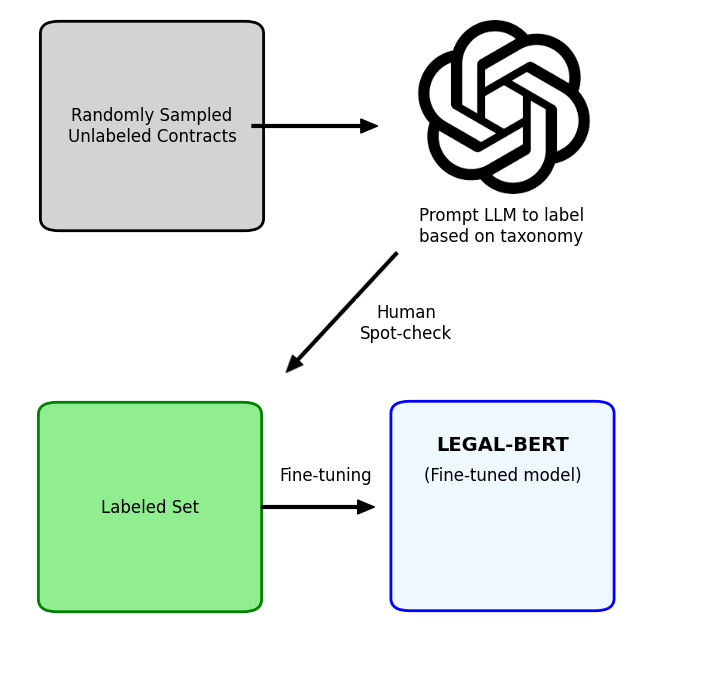
\includegraphics[width=0.6\textwidth]{llmtag.png} 
    \caption{Overview of the LLM-assisted labeling and LegalBERT training pipeline.}
    \label{fig:llm_flowchart}
\end{figure}

We first constructed a taxonomy of common legal contract types, such as Sale of Goods, Real Estate Contracts, Employment Contracts, and Licensing Agreements. Each category included clear inclusion and exclusion criteria. From a large pool of unlabeled contracts, we randomly sampled a subset(we used 5000 samples) and used GPT-4 to label them according to the taxonomy. The LLM output included predicted labels, confidence scores, and rationales. A sample of these outputs was manually reviewed to ensure accuracy.

The resulting labeled dataset was then used to fine-tune a predictive model. Prior to supervised training, we applied domain-adaptive pretraining (DAPT) by continuing masked language modeling (MLM) on the contract corpus using LegalBERT. This pretraining step used the standard cross-entropy loss over randomly masked tokens with a masking probability of 15\%. For the downstream classification task, we fine-tuned the model using weighted categorical cross-entropy, where class weights were assigned based on label frequencies to account for class imbalance, and used gradient accumulation to accommodate long sequences.

This effectively addresses the lack of labeled datasets in the legal domain by leveraging LLMs for scalable, high-quality annotation and enabling downstream training of specialized, efficient models.

\begin{table}[htbp]
\centering
\caption{Classification report on 300 testing samples}
\begin{tabular}{lcccc}
\hline
\textbf{Class} & \textbf{Precision} & \textbf{Recall} & \textbf{F1-Score} & \textbf{Support} \\
\hline
Agency Agreements & 0.3333 & 0.3333 & 0.3333 & 3 \\
Confidentiality (NDA) Agreements & 0.0000 & 0.0000 & 0.0000 & 1 \\
Construction Contracts & 1.0000 & 1.0000 & 1.0000 & 4 \\
Employment Contracts & 0.9429 & 0.7857 & 0.8571 & 42 \\
Franchise Agreements & 1.0000 & 1.0000 & 1.0000 & 1 \\
Guarantee Contracts & 0.8462 & 0.9167 & 0.8800 & 12 \\
Indemnity Contracts & 1.0000 & 0.8462 & 0.9167 & 13 \\
Insurance Contracts & 1.0000 & 0.8462 & 0.9167 & 13 \\
Lease Agreements & 0.8095 & 1.0000 & 0.8947 & 17 \\
Licensing Agreements & 0.6981 & 0.8605 & 0.7738 & 43 \\
Loan Agreements & 0.8462 & 0.9167 & 0.8800 & 24 \\
Partnership Agreements & 0.8500 & 0.7727 & 0.8095 & 22 \\
Real Estate Contracts & 1.0000 & 0.7333 & 0.8462 & 15 \\
Sale of Goods & 0.8649 & 0.9412 & 0.9014 & 34 \\
Service Contracts & 0.7027 & 0.7027 & 0.7027 & 37 \\
Settlement Agreements & 0.9091 & 0.8000 & 0.8511 & 25 \\
\hline
\textbf{Accuracy} & & & \textbf{0.8133} & 300 \\
\textbf{Macro avg} & 0.8002 & 0.7881 & 0.7902 & 300 \\
\textbf{Weighted avg} & 0.8189 & 0.8133 & 0.8113 & 300 \\
\hline
\end{tabular}
\label{tab:classification_report}
\end{table}




%=================================================



\end{document}
